\documentclass[]{report}
\usepackage{geometry}
\usepackage{graphicx}
\usepackage{physics}
\usepackage{color}
\usepackage{subcaption}
\usepackage{lipsum}
\usepackage{amsmath}
\usepackage{amsfonts}
\usepackage{amssymb}
\usepackage[hidelinks]{hyperref}
\usepackage{parskip}
\usepackage{tikz}
\usetikzlibrary{shapes.callouts, shapes.geometric, arrows}
\tikzset{
	level/.style = {
		ultra thick,
		black,
	},
	connect/.style = {
		dashed,
		black
	},
	notice/.style = {
		draw,
		rectangle callout,
		callout relative pointer={#1}
	},
	label/.style = {
		text width=2cm
	}
}
\tikzstyle{arrow} = [<->,>=stealth]

\newcommand{\up}{\fbox{$\uparrow\phantom{\downarrow}$}}%
\newcommand{\dwn}{\fbox{$\phantom{\uparrow}\downarrow$}}%
\newcommand{\updwn}{\fbox{$\mathord\uparrow\downarrow$}}%
\newcommand{\emp}{\fbox{$\phantom{\downarrow}\phantom{\downarrow}$}}%
\newcommand{\electron}[2]{{%
		\setlength\tabcolsep{0pt}% remove extra horizontal space from tabular
		      %\setlength\fboxrule{0.2pt}% uncomment for original line width
		\begin{tabular}{c}
			\fboxsep=0pt\fbox{\fboxsep=3pt#2}\\[2pt]
			#1
		\end{tabular}%
}}

%\geometry{top = 2.5cm, bottom = 2.5cm, left = 2.5cm, right = 2.5cm}
%
\setlength{\parindent}{0mm}
%\setlength{\parskip}{0.5mm}

% Title Page
\title{A Study of the t-J Model\vspace{-5mm}}
\author{Amit Bikram Sanyal}
\date{Submitted on \today}

\newcommand{\I}{\,\mathrm{i}\,}

%\let\cleardoublepage=\clearpage

\begin{document}
\begin{minipage}{\linewidth}
\maketitle
\end{minipage}
\vfill
\begin{center}
	\includegraphics[width=0.4\linewidth]{images/niser-logo}
\end{center}


\newpage
\tableofcontents
\thispagestyle{empty}

\begin{abstract}
\lipsum[1]
\end{abstract}

\chapter{The Hubbard model with strong interactions}
\section{Introduction}
The Hubbard model is one of the simplest many-body models. The one-dimensional model consists of an array of $ N $ sites with $ L $ fermions. The Hubbard model captures the effect of the electrons hopping from site to site, causing the electrons to de-localize and give rise to metallic behaviour, as well the effect of strong electron-electron interactions that cause the system to go to insulating states.

The one-dimensional Hubbard Hamiltonian with nearest-neighbour hopping is given as:
\begin{align}
\hat{H} = -t \sum_{\langle j, i \rangle } \sum_{\sigma} \left( c^{\dagger}_{j, \sigma} + c^{}_{i, \sigma} \right) + U \sum_{j} \hat{n_{i \uparrow}} \hat{n_{j \downarrow}}
\end{align}

where $ t $ denotes the hopping constant and $ U $ is the interaction energy cost when two fermions of opposite spins occupy the same site. The Hubbard model is a tight-binding model, in the sense that particles are localized on each site by Wannier functions and can only jump from site to site, without occupying any intermediate position.

\section{Spectrum of the interacting system}
The basis of a single site labelled $ i $ the Hubbard model consists of four possible states.
\begin{enumerate}
\item The empty site: $ \ket{0}_i $
\item The singly occupied site with an up spin: $ \ket{\uparrow}_i = c^{\dagger}_{i \uparrow} \ket{0}_i$ 
\item The singly occupied site with a down spin: $ \ket{\uparrow}_i = c^{\dagger}_{i \downarrow} \ket{0}_i$
\item The doubly occupied site: $ \ket{\uparrow\downarrow}_i = c^{\dagger}_{i \uparrow} c^{\dagger}_{i \downarrow} \ket{0}_i $, denotes as $ \ket{d}_i $ this point onward.
\end{enumerate}

This convention regarding $ \ket{d}_i $ has been maintained, which means $ c^{\dagger}_{i \downarrow} c^{\dagger}_{i \uparrow}  \ket{0}_i  = - c^{\dagger}_{i \uparrow} c^{\dagger}_{i \downarrow} \ket{0}_i = -\ket{d}_i $.

The spectrum of the Hubbard model is parametrized by the filling ratio, $ n = N/L $ and the relative interaction strength, $ U/t $. We shall now investigate the nature of the spectrum of the Hubbard model by varying these parameters.

First, we turn off both the hopping and the interaction, that is, we set $ t=0 $ and $ U=0 $. Let the on-site energy of each site to be $ \epsilon_0$. At $ t=0 $, each single site becomes isolated, and electrons are not allowed to hop to adjacent sites. Also Each site can be empty, or singly- or doubly-occupied. But since $ U=0 $ as well, the doubly-occupied state also does not cause any change in energy to the system. This gives rise to the single, fourfold degenerate energy level at $ E=\epsilon_0 $ for all  four occupation states.

\begin{figure}[h!]
\centering

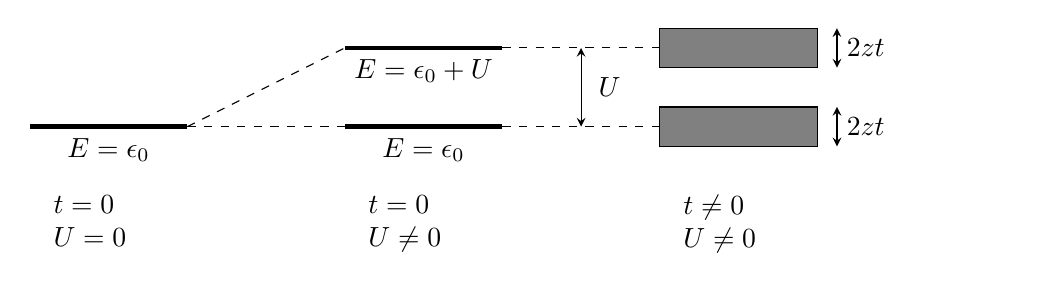
\begin{tikzpicture}
\draw[level] (0,0) -- node[below] {$ E = \epsilon_0 $} (2,0);
\draw[connect] (2, 0) -- node{} (4,0);
\draw[level] (4,0) -- node[below] {$ E = \epsilon_0 $} (6,0);
\draw[connect] (6, 0) -- node{} (8,0);
\filldraw [gray, draw = black] (8,-0.25) rectangle (10,0.25);
\draw[arrow] (10.25, -0.25) -- (10.25, 0.25);
\node[label, right] at (10.25, 0) {$ 2zt $};
\draw[connect] (2, 0) -- node{} (4,1);
\draw[level] (4,1) -- node[below] {$ E = \epsilon_0 + U $} (6,1);
\draw[connect] (6, 1) -- node{} (8,1);
\filldraw [gray, draw = black] (8,1-0.25) rectangle (10,1.25);
\draw[arrow] (10.25, 1-0.25) -- (10.25, 1.25);
\node[label, right] at (10.25, 1) {$ 2zt $};

\draw[arrow] (7,0) -- (7,1);
\node[label, right] at (7.1, 0.5) {$ U $};

\node[label, below] at (1.3,-0.75) {$ t = 0 $ \\ $ U=0 $};
\node[label, below] at (5.3,-0.75) {$ t = 0 $ \\ $ U \ne 0 $};
\node[label, below] at (9.3,-0.75) {$ t \ne 0 $ \\ $ U \ne 0 $};
\end{tikzpicture}
\caption{Degenerate bands split into two in presence of electron-electron interaction, and each band further broadens when electrons are allowed to hop.}
\end{figure}

\end{document}

